\section{Saules apstarojums}
% \begin{figure}[h]
%     \centering
%     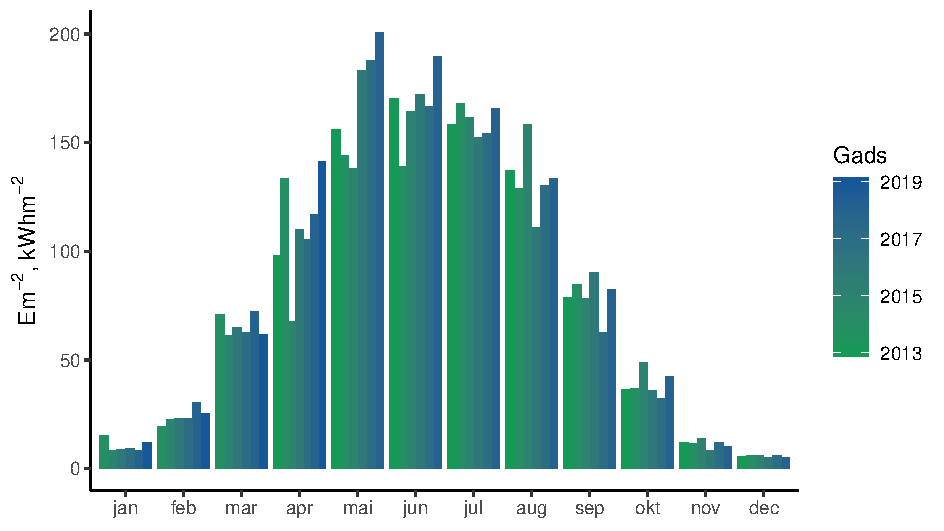
\includegraphics[width=\linewidth]{figures/meteo/statsYears.pdf}
%     \caption{Solārā apstarojuma laika integrāļa atšķirības gada gaitā. Eksperimentālā poligona meteostacijas stacijas dati 2013 -- 2019 periodā.}
%     \label{fig:metYears}
% \end{figure}

% izlabo visur lu meteoroloģiju uz poligonu
% pārsaukt grafikā Em^-2 uz E_{norm} (normētais enerģijas blīvums)

Tieši ilgtermiņa saules apstarojuma monitorings saules paneļu uzstādīšanas vietā ir svarīgs paneļu efektivitātes prognozēšanas rīks, jo ļauj izslēgt anomālu saulaina laika periodu svaru, kādi, piemēram, ir 2014. un 2019. gada aprīļi (skat. \ref{fig:metYears_mean}. att.). PV sistēmas veiktspējas monitoringam lietots Saules apstarojuma sensors (piranometrs), kas atrodas eksperimentālā poligona teritorijā. Šī mērierīce saules apstarojumu uztver ar plaknes virsmu no 180\textdegree skata leņķa, ko sauc par puslodes saules apstarojumu. Mērierīces kļūda ir  $\pm 1 \%$ ~\cite{pyranometer}.

Attēlos \ref{fig:met_Irrad} un \ref{fig:met_Irrad_mean} redzams gaišo diennakts stundu momentānā saules apstarojuma integrāļi 5 minūšu intervālos novēroto četru mēnešu laikā, kas izskaidro turpmāk minētās atšķirības paneļu ražīgumā atkarībā no mēneša -- palielinās gan Saules spīdēšanas ilgums dienā (x ass), gan saņemtās enerģijas daudzums (y ass).

\begin{figure}[h]
    \centering
    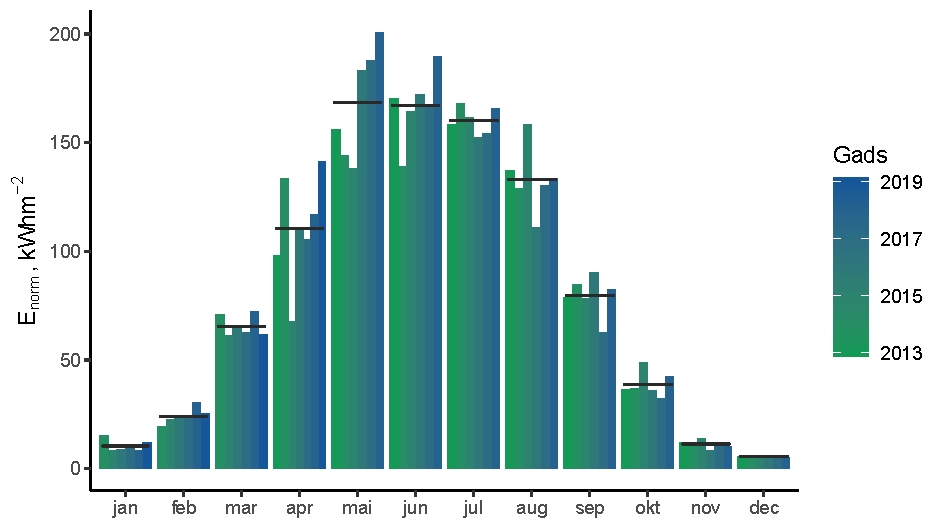
\includegraphics[width=\linewidth]{figures/meteo/meanYears.pdf}
    \caption{Solārā apstarojuma laika integrāļa atšķirības gada gaitā un to vidējās vērtības. Eksperimentālā poligona meteostacijas stacijas dati 2013 -- 2019 periodā.}
    \label{fig:metYears_mean}
\end{figure}
\begin{figure}[h]
    \centering
    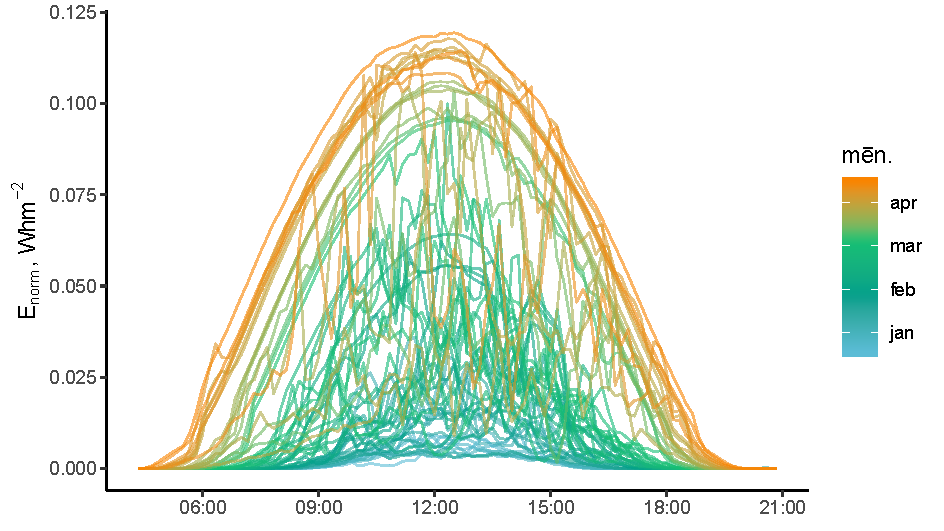
\includegraphics[width=\linewidth]{figures/meteo/sun19.pdf}
    \caption{Solārā apstarojuma izmaiņas dienas gaitā. Eksperimentālā poligona meteostacijas stacijas dati 2019-01-01 -- 2019-04-31 periodā.}
    \label{fig:met_Irrad}
\end{figure}
\begin{figure}[h]
    \centering
    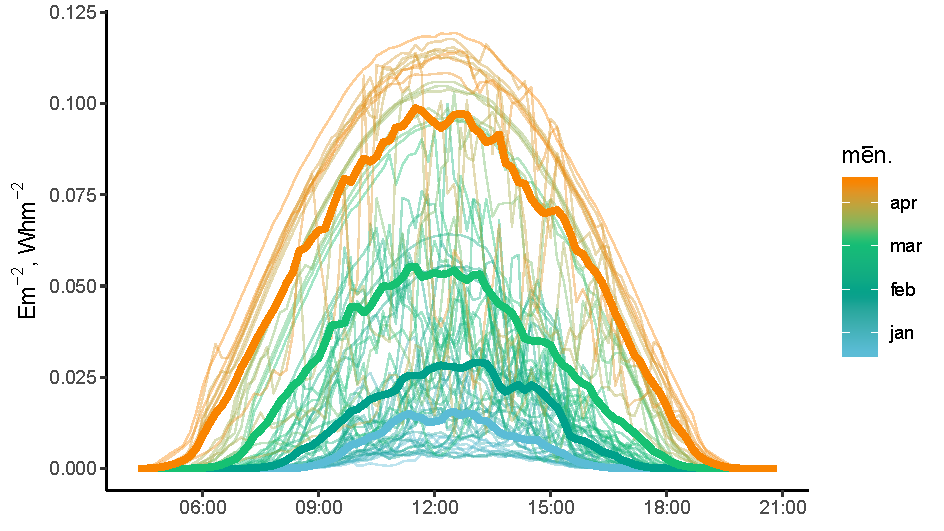
\includegraphics[width=\linewidth]{figures/meteo/mean19.pdf}
    \caption{Mēnesī vidējotas solārā apstarojuma izmaiņas dienas gaitā. Eksperimentālā poligona meteostacijas stacijas dati 2019-01-01 -- 2019-04-31 periodā.}
    \label{fig:met_Irrad_mean}
\end{figure}